\documentclass[letterpaper]{article}
\usepackage[utf8]{inputenc}
\usepackage[spanish]{babel}
\usepackage{amssymb, amsmath}
\usepackage{graphicx}
\usepackage{lipsum}
\usepackage{dsfont}
\usepackage[margin=1.5cm,
vmargin={1cm,0.3cm},
includefoot]{geometry}
\usepackage{setspace}
\usepackage{subcaption}
\usepackage{tocloft}
\usepackage{upgreek}
\usepackage{amsthm}
\usepackage{graphicx}
\usepackage{paralist}
\usepackage{fancyhdr}
\usepackage{lmodern}
\usepackage{tcolorbox}
\usepackage{color}
\usepackage{tikz}
\tcbuselibrary{skins,breakable}
\pagestyle{fancy}

\renewcommand{\headrulewidth}{0.4pt}
\renewcommand{\footrulewidth}{0.4pt}

\providecommand{\abs}[1]{\left|#1\right|}
\providecommand{\norm}[1]{\left|\left|#1\right|\right|}														  
\newcommand{\tq}{ \quad \cdot  \backepsilon \cdot \quad }

\newcommand{\ld}{\lim\limits_{x \to 0^{+}}}

\newcommand{\li}{\lim\limits_{x \to 0^{-}}}

\newcommand{\la}{\lim\limits_{x \to a}}

\newcommand{\R}{\mathds{R}}

\newcommand{\Z}{\mathds{Z}}

\newcommand{\N}{\mathds{N}}

\renewcommand{\P}{\mathcal{P}}

\newcommand{\Po}{\mathds{P}_2(\mathds{R})}

\renewcommand{\*}{\cdot}

\makeatletter
\renewcommand*\env@matrix[1][*\c@MaxMatrixCols c]{%
	\hskip -\arraycolsep
	\let\@ifnextchar\new@ifnextchar
	\array{#1}}
\makeatother

\newtheorem{theorem}{Teorema}[section]
\theoremstyle{definition}
\newtheorem{definition}{Definición}

\begin{document}
\setlength{\unitlength}{1cm}
\thispagestyle{empty}
\begin{picture}(19,3)
\put(-0.5,1.2){
\includegraphics[scale=.20]{unam1.png}}
\put(16,1){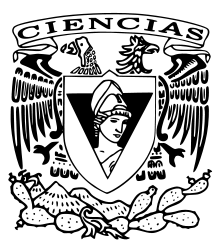
\includegraphics[scale=.29]{fciencias1.png}}
\end{picture}

\begin{center}
	\vspace{-114pt}
	\textbf{\large Álgebra Superior I}\\
	\textbf{ Semestre 2020-2}\\
	Prof. Alejandro Dorantes Aldama\\
	Ayud. Elmer Enrique Tovar Acosta \\
	Ayud. Alejandro Ríos Herrejón \\
	\textbf{Tarea III}
\rule{19cm}{0.2mm}
	\begin{center}
Kevin Ariel Merino Peña\footnote[2]{Número de cuenta: 317031326}
	\end{center}
	\vspace{-0.5cm}
\rule{19cm}{0.2mm}
\end{center}
 %%%%%%%%%%%%%%%%%%%%%%%%%%%%%%%%%%%%%%%%%%%%
 %			|	EJERCICIO 5					%
 %			|	ARIEL						%	
 %%%%%%%%%%%%%%%%%%%%%%%%%%%%%%%%%%%%%%%%%%%%
\noindent5.Enliste todas las ordenaciones de las letras $ a, b, c, d $ tomadas de tres en tres.\\
$$ \begin{array}{cccccc}
abc & adb & acd & acb & adc & adb\\
bca & bcd & bda & bdc & bad & bac\\
\end{array} \hspace{2cm} \begin{array}{cccccc}
cad & cab & cbd & cba & cda & cdb\\
dab & dac & dbc & dba & dca & dcb\\
\end{array}$$
 %%%%%%%%%%%%%%%%%%%%%%%%%%%%%%%%%%%%%%%%%%%%
%			|	EJERCICIO 9					%
%			|	ARIEL						%	
%%%%%%%%%%%%%%%%%%%%%%%%%%%%%%%%%%%%%%%%%%%%
\noindent9.Escríbanse todas las permutaciones de los dıgitos $ 1, 2, 3, 4 $\\
\[
\begin{array}{cccccc}
 1234& 1243 & 1342 & 1324 & 1423 & 1432 \\
 2134 & 2143 & 2341 & 2314 & 2413& 2431\\
\end{array} \hspace{2cm} \begin{array}{cccccc}
 3124 & 3142 & 3241 & 3214 & 3412& 3421\\
4123 & 4132 & 4231 & 4213 & 4312 & 4321\\
\end{array}
\]

 %%%%%%%%%%%%%%%%%%%%%%%%%%%%%%%%%%%%%%%%%%%%
%			|	EJERCICIO 15				%
%			|	ARIEL						%	
%%%%%%%%%%%%%%%%%%%%%%%%%%%%%%%%%%%%%%%%%%%%
\noindent15.Un juego de dominó consta de 28 fichas y una mano consta de 7 fichas.
¿De cuántas formas se puede seleccionar una mano?\\
Para ello podemos ocupar, de las notas que 
\[ C_n^m = \dfrac{n!}{m!(n - m)!} \]así obtendremos el número de combinaciones posibles de 7 en 7 en 28 elementos
\begin{align*}
	C_{28}^7 &= \dfrac{28!}{7!(28 - 7)!} & C_{28}^7 &= \dfrac{28\* 27 \* 26 \* 25 \* 24 \* 23 \* 22 \* 21!}{7!21!}\\
	C_{28}^7 &= \dfrac{28!}{7!21!} & 	C_{28}^7 &= \dfrac{28\* 27 \* 26 \* 25 \* 24 \* 23 \* 22 }{7!}\\
	&  & C_{28}^7 &= 1184040
\end{align*}
\begin{center}
	$ \therefore $ tenemos 1184040 formas de seleccionar una mano cuando jugamos dominó $ :) $
\end{center}
 %%%%%%%%%%%%%%%%%%%%%%%%%%%%%%%%%%%%%%%%%%%%
%			|	EJERCICIO 18				%
%			|	ARIEL						%	
%%%%%%%%%%%%%%%%%%%%%%%%%%%%%%%%%%%%%%%%%%%%
\noindent18.¿Cuántas manos de póker hay que tengan exactamente una tercia y que no sea un full? Justifique su respuesta.\\
Para conseguir una tercia en póker, tenemos $ C_3^4 $ formas de obtenerla, luego como son 13 cartas que hay por cada figura, entonces la posiblidad de tener una tercia (cualquiera) es $ 13 C_3^4  $.\\
Para evitar que sea un \textit{full}, se pide que las otras dos cartas sean distintas entre sí, entonces existen $ 48 $ opciones para la $ 4^{ta} $ carta elegida y para la última carta sólo quedan $ 44 $ posibilidades, entonces:
\begin{align*}
	13 C_3^4 (48)(44) &= 13 \left( \dfrac{4!}{3!(4-3!)} \right)(48)(44)\\
	13 C_3^4 (48)(44) &= 13(4)(48)(44)\\
	13 C_3^4 (48)(44) &= 109824
\end{align*}
\begin{center}
	$ \therefore $ Como no nos importa el orden de las últimas dos cartas entonces existen $ \frac{109824}{2} = 54912  $ maneras de conseguir una tercia y que no sea un full.
\end{center}
 %%%%%%%%%%%%%%%%%%%%%%%%%%%%%%%%%%%%%%%%%%%%
%			|	EJERCICIO 23				%
%			|	ARIEL						%	
%%%%%%%%%%%%%%%%%%%%%%%%%%%%%%%%%%%%%%%%%%%%
\noindent23.¿De cuántas formas diferentes es posible ordenar los símbolos $ s,a,r,a,s,e,r,a $?\\
La respuesta es $ \dfrac{8!}{3!2!2!} =1680 $ esto es porque no se necesitan ordenar 8 elementos diferentes para obtener las 1680 ordenaciones distintas.\\

 %%%%%%%%%%%%%%%%%%%%%%%%%%%%%%%%%%%%%%%%%%%%
%			|	EJERCICIO 30				%
%			|	ARIEL						%	
%%%%%%%%%%%%%%%%%%%%%%%%%%%%%%%%%%%%%%%%%%%%
\noindent30.¿Cuántas ordenaciones de las letras de \textit{PRINCIPIO} no tienen I consecutivas?\\
Si no tomamos en cuenta las letras \textbf{I}, existen $ \dfrac{6!}{2!} = 360 $ ordenaciones con las letras restantes, entonces dichas ordenaciones se verían de la siguiente forma $ PPRNCO $, por dar un ejemplo, observemos que hay 7 espacios donde poner $ I $, debemos elegir 2 de estas posiciones al colocar las letras $ I $, \textit{i.e.} $ C_2^7 = \dfrac{7!}{2!(5!)} = 21 $
\begin{center}
	$ \therefore  $ hay $ 360 \* 21 $ ordenaciones de $ PRINCIPIO $ que no tienen $ I$ consecutivas.
\end{center}
\end{document}